\actTitle{2.1 Part 1 - Quadratic Functions and Applications}


\noindent \textbf{Topics:}  quadratic functions, standard equation for  a quadratic, and vertex of a parabola\\

\noindent \textbf{Student Learning Outcomes:}
\begin{enumerate}
\item Students will be able to recognize quadratic functions graphically and algebraically.
\item Students will be able to write the standard equation for a quadratic function.
\item Students will be able to determine the vertex of a parabola.
\end{enumerate}

\hrule 

\bigskip

\subsection{Standard Form of a Quadratic Function} ~

\noindent \underline{Quadratic Formula.} The roots of the equation $ax^2+bx+c=0$ are \begin{tabular}{| l |} \hline \\ $x = \dfrac{-b \pm \sqrt{b^2-4ac}}{2a}$  \\ \\ \hline
\end{tabular} 


\hspace{-.3in}\begin{tabular}{| l |} \hline 
\noindent \underline{Standard Equation of a Parabola.} The standard equation of a parabola is \\
$ y = a(x-h)^2 + k$. The point $(h,k)$ is the vertex of the parabola.
\\ \hline
\end{tabular} 

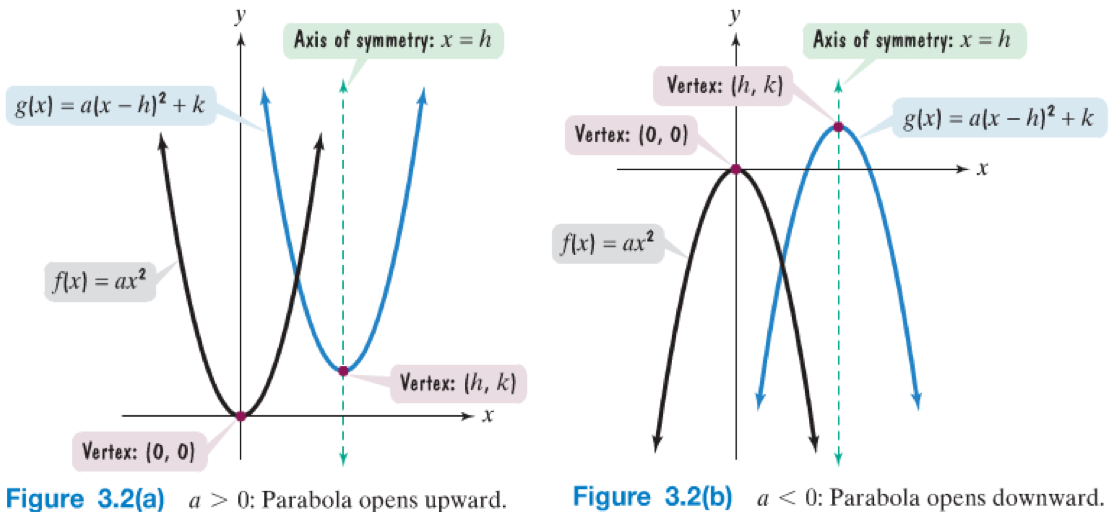
\includegraphics[scale=.7]{graphstandard}



\newpage


\subsection{Graphing a Quadratic Function in Standard Form}

\begin{enumerate}
\item The graph of a quadratic function is given.  Select the function's equation.\\
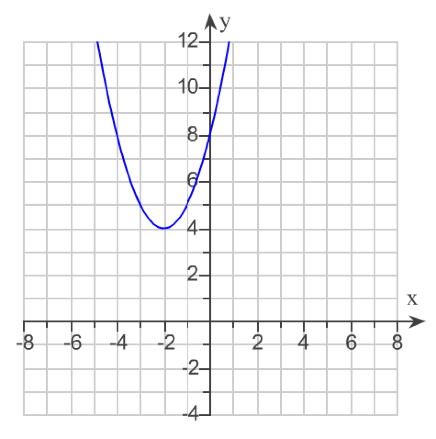
\includegraphics[scale=.7]{quad1a}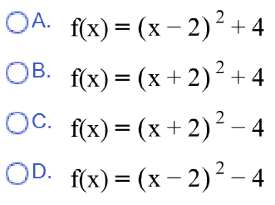
\includegraphics[scale=.7]{quad1b}\\
\item Given $f(x)=-2(x-1)^2+8$
\begin{enumerate}
\item Determine whether the graph of the parabola opens upward or downward.\\[.3in]
\item Identify the vertex.\\[.3in]
\item Determine the $x$-intercept(s).\\[1in]
\item Determine the $y$-intercept.\\[.5in]
\item Sketch the function.\\
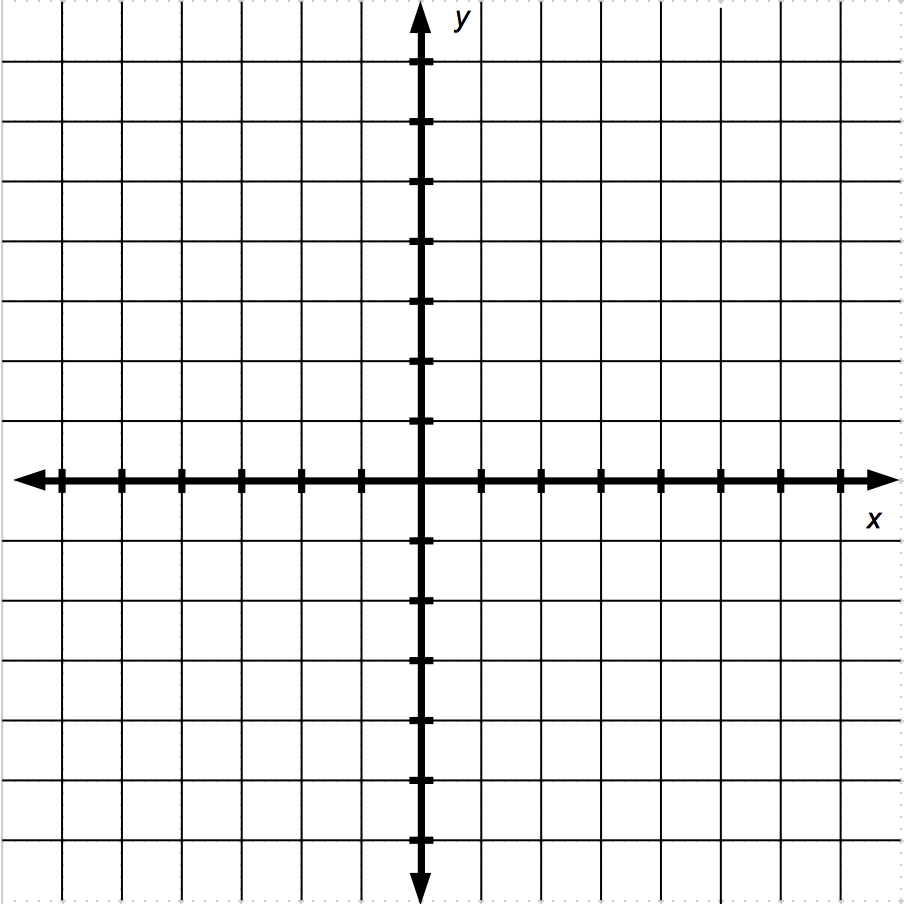
\includegraphics[scale=.5]{bigaxes}\\
\item Determine the axis of symmetry.\\



\end{enumerate}






\newpage



\subsection{Determining the Standard Form of Quadratic Function}

\noindent To determine the standard form of a quadratic function written in the form $y=ax^2+bx+c$, we use a process called \textbf{Completing the Square}.


 
 \item Determine the standard equation of the parabola $y=3x^2+12x+5$.  Then determine the vertex.
 
 
 \vfill
 
  
 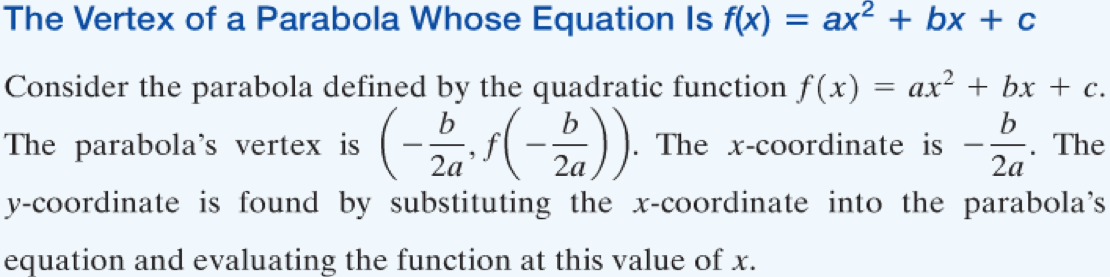
\includegraphics[scale=.75]{parabola}






\end{enumerate}

\noindent \textbf{Student Learning Outcomes Check}

\begin{enumerate}
\item Are you able to recognize quadratic functions graphically and algebraically?
\item Can you write the standard equation for a quadratic function?
\item Are you able to determine the vertex of a parabola?


\end{enumerate}

\noindent \textbf{If any of your answers were no, please ask about these topics in class.}


